In this part of the system three datasets were generated, which are a training set for Stochastic Gradient Descent algorithm, a validation set for feature selection, and a testing set. Each set consisted of three different image types: the original images, those after the process of colour quantisation and the ground truth representing the expected labelling. Figure
\ref{fig:nonlinear_testset_noise_free} presents five sample images of each type that were generated for this experiment.
The first column depicts original images that are to be segmented, which contain regions coloured with various shades of red, green and blue. On every image there is one red object on a green neighbourhood. The main goal of this experiment is to detect if a given superpixel is a part of an object with a shape of a letter H or a part of a different object. Next column presents images with a reduced colour palette, which are to simulate the result of division into textons. The last type of images represents the expected result. In this part of the system classification is done into four classes. Label 0 should be assigned to red regions which are not a part of a letter H. Label 1 and 2 are for green and blue segments respectively. The last class, marked with label 3, is devoted to objects in a shape of a letter H. On images representing the ground truth, regions with label 0 ale black, with label 1 are white, and grey colour is reserved for label 2. The last label is marked with magenta colour. 

\begin{figure}[!htb]
 \centering
    \begin{tabular}{ccc}
        \textit{original image} & \textit{colour quantisation} & \textit{expected results} \\
        \fcolorbox{black}{white}{\includegraphics[width= 0.22\textwidth]{nonlinear_noise_free/init/3.png}} &
        \fcolorbox{black}{white}{\includegraphics[width = 0.22\textwidth]{nonlinear_noise_free/test/3.png}} &
        \fcolorbox{black}{white}{\includegraphics[width = 0.22\textwidth]{nonlinear_noise_free/result/3.png}} \\
        \fcolorbox{black}{white}{\includegraphics[width = 0.22\textwidth]{nonlinear_noise_free/init/5.png}} &
        \fcolorbox{black}{white}{\includegraphics[width = 0.22\textwidth]{nonlinear_noise_free/test/5.png}} &
        \fcolorbox{black}{white}{\includegraphics[width = 0.22\textwidth]{nonlinear_noise_free/result/5.png}} \\
        \fcolorbox{black}{white}{
\includegraphics[width = 0.22\textwidth]{nonlinear_noise_free/init/6.png}} &
        \fcolorbox{black}{white}{
\includegraphics[width = 0.22\textwidth]{nonlinear_noise_free/test/6.png}} &
        \fcolorbox{black}{white}{
\includegraphics[width = 0.22\textwidth]{nonlinear_noise_free/result/6.png}} \\
        \fcolorbox{black}{white}{\includegraphics[width = 0.22\textwidth]{nonlinear_noise_free/init/9.png}} &
        \fcolorbox{black}{white}{\includegraphics[width = 0.22\textwidth]{nonlinear_noise_free/test/9.png}} &
        \fcolorbox{black}{white}{\includegraphics[width = 0.22\textwidth]{nonlinear_noise_free/result/9.png}} \\
        \fcolorbox{black}{white}{\includegraphics[width = 0.22\textwidth]{nonlinear_noise_free/init/13.png}} &
        \fcolorbox{black}{white}{\includegraphics[width = 0.22\textwidth]{nonlinear_noise_free/test/13.png}} &
        \fcolorbox{black}{white}{\includegraphics[width = 0.22\textwidth]{nonlinear_noise_free/result/13.png}} \\
    \end{tabular}
    \caption{Sample images generated for the problem of segmentation by shape on a noise-free case.}
    \label{fig:nonlinear_testset_noise_free}
\end{figure}